\section{Planning and execution in the \rx architecture}
\label{sec:arch}

% {\em\tiny This section introduces shortly T-REX architecture but move
%   quickly the focus on a single reactor and gross concepts on the
%   architecture:
%   \begin{itemize}
%   \item For t-trex the whole decision and control problem is reduced
%     around the state variables (or timeline construct). 
%   \item This reduce the execution tracking problem for each reactor on a state
%     identification problem (deduce internal state from the external
%     state), and the control problem to goal posting which will trigger
%     deliberation on the owner of the corresponding timeline. 
%   \item the architecture itself see each reactor as a black box and
%     therefore each reactor can implement its own mechanism in order to
%     resolve both synchronization and deliberation. Still we provide a
%     reactor based on the europa framework that leverage the automated
%     planning capabilities in order to do model based planning and
%     execution with a rich representation of resources and time.
%   \end{itemize}}

\subsection{Introductory concepts}
\label{sec:arch:intro}

A prime motivation behind the \rx architecture was to design a
controller which could bring automated planning closer to low-level
control of the vehicle while maintaining its reactivity. Traditionally
planning has been deemed computationally expensive with planner
performance restricting robot reactivity
\cite{ghallab04,Dias:2003ua}. In control architectures where task
planning is embedded, planning consequently remains at an abstract
level with the assumption that it would otherwise impede system
reactiveness and that the environment can change at a faster rate than
the planner can plan for it. In such a situation, the agent may thrash
if the internal state of the plan gets out of synch with the actual
state of the world. As a result the planning problem managed {\em in
  situ} remains fairly detached from low-level control. Most
adaptations at the lower-level reactive layers in contrast are managed
by specialized components (for example GeNoM \comment{} and CLARATy
\comment{}) that rely on different representations for modeling local
control behavior or worse do not have any explicit formal agent
behavior model. The consequent different techniques for specifying
each layer in the architecture results in duplication of effort and a
diffusion of knowledge leading to significant design and integration
issues \cite{DS1report}.  \texttt{IDEA} mitigated most of these issues
by tightly integrating planning and execution in a single
representational and computational framework with a unified
declarative model. Our approach with \texttt{T-REX} builds on this
design methodology albeit in a substantially systematic manner

The \rx architecture contributes to agent architectures over and
beyond \texttt{IDEA} are in the following ways:

\begin{itemize}

\item \emph{Partitioning} the global planning problem into multiple
  decision loops, called {\em reactors}. Each reactor has its own
  scope both functionally (one for example focusing on the conversion
  of high level waypoints into low-level commands) and temporally as
  each reactor declares its planning look-ahead and expected latency
  before being able to produce plan to the agent depending on where it
  is located in a reactor dependency graph such as shown in
  Fig. \ref{fig:agent}.

\item \emph{Coupling} a tighter integration between the planning
  process and world evolution to ensure that planning occurs while
  being continuously informed of state change. By doing so, the
  planner is better informed in its deliberation despite a larger
  latency than changing world change state.

\end{itemize}

Partitioned inference is a major contribution of \rx. However that is
not the focus of this chapter; details are in \cite{py10} and
\cite{rajan12}. Coupled interaction between planning and the world on
the other hand, has a significant implication on how planning can be
integrated in such frameworks; here we show using the \eu planner can
be coupled to our framework. First we link concepts in \eu planning
with the \rx framework. Note that in the following treatise, we call
the formal semantic framework of \rx as the 'agent'. Reactors
constitute an entity within this agent and are standalone blocks of
inference.

% on should integrate a
% planner in this framework in general and was applied to the europa
% framework specifically. We'll develop later how this requirement
% implies to see in-situ planning as two parallels processes that are
% tightly linked through the same plan structure. But before that we
% need to introduce at least the high leve lconcepts and ideas behind
% our architecture as a whole.

\subsection{Architectural concepts in \rx}
\label{sec:arch:trex}

The \rx architecture is structured around the notion of \eu {\em state
  variables} as the fundamental basis of interaction. Additionally it
comes with a well-defined ownership model associated with each state
variable. In this framework each reactor is seen as a 'black box'
providing its own {\em internal} state variables which it is
responsible for in order to maintain its value at every instant of
time. Each such instance is represented by a {\em tick} with a fixed
duration; in our implementation of \rx on the Dorado, we use a tick of
$1$ second. In order to identify its state a reactor can subscribe to
{\em external} state variables owned by other reactors, for which it
will receive new updates when the owner reactor generates its {\em
  internal} state.

This {\em synchronization} process propagates up through the reactor
dependency graph bottom up at every {\em tick} ensuring that all the
reactors have a consistent view of the world. Conversely each reactor
can request a future change on one of its {\em external} state
variables which will be transfromed as an {\em internal} goal to the
owner. Such \emph{goal dispatching} is expected to produce a
deliberation phase for the receiving reactor which can cyclically and
in turn, produce a plan impacting its {\em external} state variables
that will propagate down following the same mechanism.

% Taking cues from the IDEA 
% architecture \cite{mus02}, we designed a core framework that provides a
% formal basis \cite{Py:2010ti} on the way each of the sub-component --
% called reactors -- of our agent can interact by exchanging only
% information through {\em state variables} by ensuring that state 
% information can propagate through all the reactors ensuring a
% consistent view of the present state of the world at every single tick
% trough a bottom-up {\em synchronization} flow and collaboration for
% future state evolution by timely exchanges of goals on {\em state
%   variables}. This exchange does not impose to any reactor to be aware
% of the reactors it is connected to but only focus on the state
% variables it relies on (called {\em external}) and the state
% variables it manages and maintains (called {\em internal}). 


\begin{figure}[!htb]
 \centering
 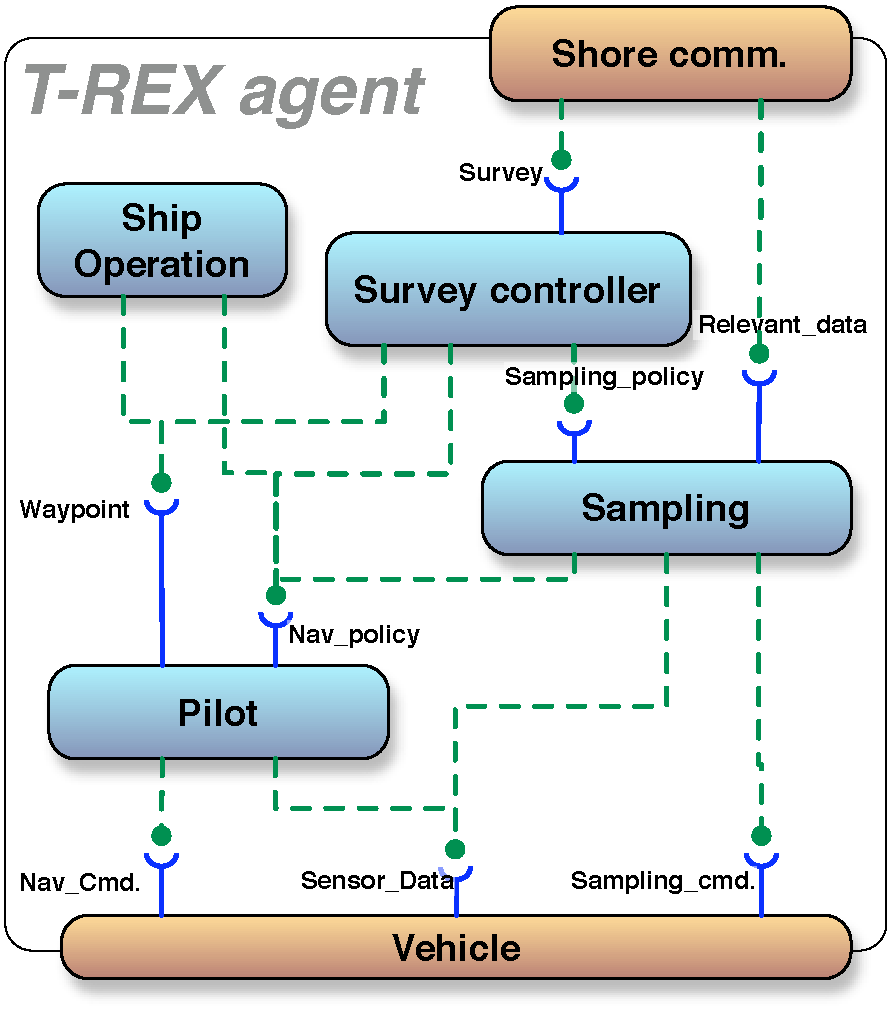
\includegraphics[scale=0.45]{figs/AUV-agent.pdf}
 \caption{\small A \rx agent is composed of multiple reactors or
   control loops (rounded boxes) which are connected through state
   variables provided by one reactor ({\color{blue}blue} solid line)
   with multiple possible clients ({\color{green}green} dashed lines)}
  \label{fig:agent}
\end{figure}

Consider for example the \rx agent instance we use on our AUV as shown
in Fig. \ref{fig:agent}. In this instance all the reactors (symbolized
by colored boxes) do not have an explicit connection from one to
another but instead rely on a publish/subscribe model on shared state
variables. For instance the \textsf{Pilot} reactor needs the {\em
  externally} managed state information from \textsf{Sensor\_Data} and
\textsf{Nav\_cmd} state variables in order to maintain the
\emph{internal} state variables \textsf{Waypoint} and
\textsf{Nav\_policy}. This relation applies in two ways:

\begin{itemize}

\item In order to identify its current {\em internal} state values the
  \textsf{Pilot} \comment{double check this mod} needs to know the
  current {\em external} state information it relies on. In this case
  the current \textsf{Waypoint} the vehicle is heading to can be
  extracted for example from the current \textsf{Nav\_cmd} executed.

\item The future objectives a reactor has on \textsf{Internal} state
  will likely imply sub-objectives to be reported to the owner of its
  {\em external} state variables depending on their current
  values. Should the \textsf{Pilot} want to visit a specific
  \textsf{Waypoint} -- given its current position as provided by
  \textsf{Sensor\_Data}, it can identify a sequence of
  \textsf{Nav\_cmd} states that should eventually help it reach this
  location. \comment{this explanation could do with a figure which I
    believe we have used previously}

\end{itemize}

Given the above example, the \rx architecture therefore helps abstract
reactor interaction by constraining them to state variables. Each
reactor is therefore agnostic where its {\em external} state
information is managed as long as this information is available and
properly maintained for managing {\em internal} state
information. This {\em internal} state in turn may be used by other
reactors. Such a formalism also constrains reactor interaction to
state information exchange which comes in two forms:

\begin{itemize}

\item {\em Observation on current state values}: This information
  propagates \emph{up} in the reactor dependency graph at the
  synchronization phase and occurs at the beginning of every
  tick. During this phase the agent provides updates to each reactor
  on their {\em external} state variables for this tick so as they
  could compute their {\em internal} state variable values for this
  same tick. By doing so we propagate a consistent view of that state
  of the world throughout all the reactors as time
  advances. \comment{could do with a figure here}

\item {\em Goal request on future state}: This information propagates
  \emph{down} in the reactor dependency graph. In order to satisfy own
  {\em internal} objectives, a reactor may have a plan that relies on
  future values of one of its {\em external} state. When such a plan
  is identified the agent ensures that this part of the plan is given
  as a goal to the owner of the given {\em external} state
  variable(s). \comment{could do with a figure here}

\end{itemize}

The choice of representation of state variables, observations and
goals is directly derived from \eu timelines and tokens.  While such a
rich representation allows exchange of state information in a formal
yet flexible manner, its translation into planning frameworks that
have an explicit representation of time (such as but not limited to
\eu) is often trivial.

\subsection{The Execution Cycle}
\label{sec:arch:exec}

The overall execution cycle of the agent is also abstracted out as a
continuous planning/deliberation cycle between all reactors. At the
agent interface level, each reactor provides only two abstract calls
that conceptualize execution:

\begin{itemize}

\item \texttt{synchronize} takes the last {\em external} observations
  as an argument and returns the {\em internal} observations for a
  reactor or a failure report.

\item \texttt{step} that accepts new goals requested (if any) on the
  {\em internal} timeline of a reactor and will execute one step of
  deliberation \comment{Might be good to articulate what ``one'' step
    looks like}. The returned value indicates if a complete plan has
  been found. If so this part \comment{what does 'this part' mean? Can
    we sketch a figure or make it more formal?} of the plan is
  provided to {\em external} timelines of this reactor.

\end{itemize}

Both these deliberative functions have different scope and temporal
constraints. The \texttt{synchronize} call is considered as atomic and
will focus only on state inference for the current tick by identifying
the current value of {\em internal} state variables from the latest
updates on the {\em external} state variables. This process propagates
up in the reactor dependency graph at every tick to ensure that all
reactors are aware of the current state of the world. \texttt{step}
relates to a single decision step of the planning process which is
focused on the future evolution of state variables; it can take
multiple steps spanning multiple ticks for a reactor to produce a plan
that is both complete and valid. When such plan is identified
\comment{how? Is there a terminating condition?} its {\em external}
timeline(s) are then dispatched to the corresponding reactors which
own these times and which in turn can start their own deliberation
\texttt{step}s to satisfy these new objectives. Consequently execution
occurs as these goals and plans propagate down in the reactor
hierarchy until they eventually become goals for the lowest level
reactor which -- instead of deliberating -- may just transform this
goal into a command for execution in hardware.

\begin{figure}[!htbp]
  \centering
  \vskip-1pc
  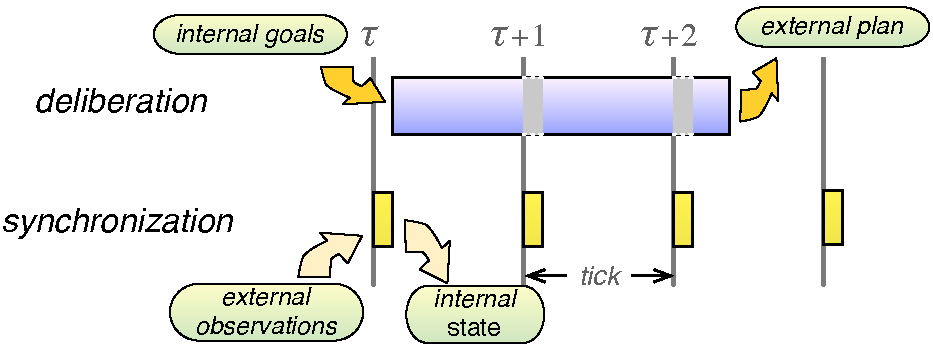
\includegraphics[width=0.55\columnwidth]{figs/tick-cycle}
  \caption{\small \rx reactor execution cycle: {\em Deliberation} is
    interrupted by {\em synchronization} at the beginning of every
    {\em tick} allowing integration of state information.}
  \label{fig:tick-exec}
  \vskip-0.8pc
\end{figure}

The manner in which the agent interleaves planning \texttt{step}s and
synchronization for a single reactor is illustrated in
Fig.~\ref{fig:tick-exec}. Synchronization occurs at every tick while
interrupting planning; this allows a reactor to identify its current
state that can propagate through the reactor hierarchy in order to
ensure a consistent view of the state of the world between all the
reactors.
% This view of a reactor has two parallel tasks allowing for long
% planning deliberation while ensuring that the state evolution
% propagates through the agent as time advance.
These intertwined tasks together provide two natural information flows
(bottom-up for state estimation and top-down for plan projection) that
we expect to see in a control loop. As they are both inference-based
processes it is natural to implement a reactor based on generic
automated planning. For example in Fig. \ref{fig:agent}, apart from
\textsf{Shore comm.} and \textsf{Vehicle} acting as interfaces to the
system, every other reactor (in blue) are different instances of a \eu
reactor differentiated only by their model and \eu solver
configurations.

\subsection{The  \eu Deliberative Reactor}
\label{sec:arch:europa}

Within \rx, an instance of an \eu reactor comes with the sole purpose
to deliberate. A typical design of such a reactor takes its cues from
\texttt{IDEA} \cite{mus02, mus06} where both planning and execution
are based on a single unified model within a rich representation that
provides support for temporal inference. In \rx, the execution cycle
consists of two deliberation processes which are implemented as two
\eu solvers modifying the \emph{same} plan database. %  and for which the
% execution is managed by the \rx framework as time advance during the
% execution of the system:

\begin{enumerate}

\item The \emph{synchronization solver} is a specialized \eu solver
  that integrates new information in the plan, the evolution of
  \emph{external} state variables and ensures that the reactor
  propagates these to identify the reactors current state as well as
  to inform other reactors of any state change on its \emph{internal}
  timelines. This solver is summoned at the beginning of every single
  tick.

\item The \emph{deliberation solver} manages the deliberation process
  of the reactor either to produce a new plan or alter its current
  plan as new goals are provided or when the synchronization solver
  identifies a conflict between current state and expectations from a
  previously generated plan. This process can span multiple ticks and
  can therefore be interrupted by the synchronization solver.

\end{enumerate}

While the two processes are separate, they share the same plan
internal to a reactor; consequently at every synchronization cycle the
planning process is informed of the new world state and its impact on
the plan. Conversely, when the deliberation process eventually finds a
solution, synchronization is informed about generating the planned
state values \comment{should this read as ``...is informed about
  generated state values..'' instead?} on the {\em external} state
variables. This {\em external} plan defines the set of {\em goals} for
this state variable managed by another {\em reactor}.

Synchronization offers an important challenge for embedding planning
in a situated agent, typically %  as always been to go around the asumptions made by
% most classical planners. Specifically one
an assumption to restrict the problem to ``offline planning'' defined
in \cite{ghallab04} as follows:

\begin{quotation}
  The planner is not concerned with any change that may occur in
  $\Sigma$ \footnote{the world modeled by the plan domain} while it is
  planning; it plans for the given initial and goal states regardless
  of the current dynamics, if any. 
\end{quotation}

This assumption, while helpful to reduce the scope of the planning
problem, becomes problematic for planning within a highly dynamic
environment. In a typical robot this implies that the only point where
the planner can be informed about the current world state is prior to
the commencement of a planning cycle by giving to the planner the
initial state and current objectives. During the planning, it is
assumed that the agent can maintin the world as perceived by the
planner as stable. \cite{lemai04, lemai-chenevier2004} attempts to
reduce the impact of planning by allowing local plan repair in the
existing plan. In the eventuality that such repair is not feasible
they require that their robot comes to a full stop until (re-)planning
is complete. \comment{I may need more examples/refs here}. As Fig.
\ref{fig:tick-exec} shows, this assumption is problematic for our
architecture. Synchronization that tracks state evolution can occur
several times during the reactor deliberation process. By making
synchronization and deliberation share the same plan we provide a
solution that relaxes this static world assumption. 

In the following sections we show how synchronization and deliberation
are implemented independently to show how their interaction through
the plan helps relax this assumption by making planning fully
integrated in the reactor execution cycle while potentially allowing
for more informed planning.

\subsubsection{Synchronization identify internal state evolution}
\label{sec:arch:synch}

\begin{figure}[!htbp]
  \centering
  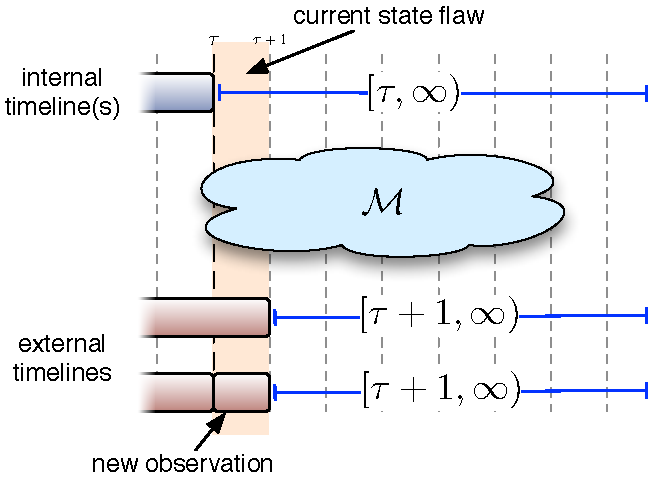
\includegraphics[width=0.5\columnwidth]{figs/synch-relation}
  \caption{\small Illustration of the synchronization flaws in a reactor. The
    reactor receive new observations when they are produced by the
    owner(s) of its internal timelines. The line after the last token
    of each timeline represent the domain of possible values for the
    end of this token. At every tick $\tau$ the reactor needs to
    integrate the {\em External} state information it received and --
    based on its model $\mathcal{M}$ -- resolve its {\em Internal}
    state that will then be provided by the architecture to other
    reactors using these state variables.}
  \label{fig:synch:flaw}
\end{figure}

We first show how a reactor can track and identify its state in the
context where it does not have any compelling need to deliberate. We
assume that we have a reactor that has no future goal. \comment{Need
  to develop the reason why it is a necessity: primarily to provide
  its internal state to whoever observe it but also simply to ensure
  that its current representation of the world is up to date and still
  consistent}

We introduce this requirement as a new type of flaw (Section
\ref{sec:europa:arch}) for the \eu framework. This flaw forces the
reactor to identify its internal state for the current tick. By using
this flaw one can describe the synchronization process as:

\begin{enumerate}

\item Integrate the external state as provided by the owner of each
  external timeline into the plan database.

\item Propagate this information in the plan database following the
  model $\mathcal{M}$ of this reactor.

\item Resolve the current state value of each internal timelines.

\end{enumerate}

An internal state flaw can be resolved using one of the following
choices which are evaluated in order:

\begin{enumerate}

\item Extend the previous state value to end after this tick (\ie
  restrict its end time to $[\tau+1, \infty)$). \comment{first use of
    $\tau$, so needs to be defined earlier}

\item Start the next active token in the timeline 
  by restricting its start time to the single value $\tau$

\item Create and insert a new token in this timeline that will start
  at the current tick $\tau$ (attempt this for each possible token
  type for this timeline if necessary). 

\end{enumerate}

All of these choices are evaluated sequentially until a consistent
solution with no flaws at this tick, is identified. In order to do so
we need to make the assumption that the current state value of an
internal timeline does not depend on the future or more accurately
that any choices made during this synchronization will not lead to a
future inconsistency. Such an assumption impacts the set of possible
domains the reactor can support while remaining complete. Take for
example this rule from our \texttt{Shopping} model :

\begin{verbatim}
 1 Agent::Go {
 2   met_by(condition object.location.At origin);
 3   eq(from, origin.loc);
 4
 5   equals(effect object.location.Going going);
 6   eq(going.from, from);
 7   eq(going.to, to);
 8   
 9   meets(effect object.location.At destination);
10   eq(to, destination.loc);
11 }
\end{verbatim}

While this model is perfectly standard and acceptable in the overall
case. It can become problematic when tied to execution. Specifically it
puts a strong tie between the {\em fact} that we are \texttt{Going} to a
location and the {\em expected} future outcome of ending at this
location. This ties is even stronger due to the constraint at line 5.
Knowing this aspect assume that the \texttt{Agent.location} is {\em
  external} to the reactor which receive the observation
\texttt{Going(Home,SuperMarket)} which synchronization resolved by
producing the observation \texttt{Go(Home, SuperMarket)} in the Agent
timeline. From this point this means that the only possible outcome on
\texttt{Agent.location} is to be \texttt{At(SuperMarket)} in the
directly foreseeable future. In the real world the fact that we are
\texttt{Going} to a certain location does not necessarly imply that we
will succeed on ending up there. An extreme case could be that due to
some exogenous event, the road to the \texttt{SuperMarket} is closed
which could result on an alternate observation \texttt{At(7th st. \& Foo
  Ave.)}. This observation contradicts thre existing plan the reactor
maintin and it is important here to relaize the temp[oral direction of
the causal link that is triggereing this inconsitency. Indeed at the
time we will observe this contradicting \texttt{At}, the rule that
generated this conlict is connected to the past observations
\texttt{Going} and \texttt{Go} which cannot be fully retracted without
potential global impact in the rest of the exisiting reactors --
implying a huge cost in backprogation that would be problematic.

More generally tying a token to future outcomes in a model that is meant
to be confronted to rela 
executionis something that is problematic. It may be valid ifg you can
gurantee that this will always happen (for example the reactor
managing \texttt{Agent.location} timeline guarantees that the outcome
of the \texttt{Going} will {\em always} result on ending at the traget
location) but should be manipulated while keeping in mind that
predicting the future is not absolute. In this case one could alter
this part of the model as follow in order to give the reactor more
flexibility:

\begin{verbatim}
 1 Agent::Go {
 2   met_by(condition object.location.At origin);
 3   eq(from, origin.loc);
 4
 5   contains(effect object.location.Going going);
 6   eq(going.from, from);
 7   eq(going.to, to);
 8   
 9   meets(effect object.location.At destination);
10   eq(to, destination.loc);
11   going meets destination;
12 }
\end{verbatim}

The alteration made to relax the constraint on linbe 5 from a strict 
\texttt{equals} to contains and then add the new constraint at line 11
that ensure that the last \texttt{Going} done during this \texttt{Go}
ends up in the location the agent wnats to be. This firts level of
relaxation will therefore allow the agent to usies multiple
\texttt{Going} should the first one fail to reach our objective.  The
probalem can even be relaxed further if needed but this relaxation
gicves already more felxibility for the reactor to recover from local
failures.

Synchronization remains here a deliberation process, and for this
reason there's always the risk that the search of a solution is not a
straightforward sequence of unit decision. As such process is required
by the architecture at every ticks for every reactors presently
running this need to be carefully designed. At the engine level we
made careful choices in term of both the focus of the search --
limited only to tokens that can potentially overlap the current tick
-- and its heuristic where the internal state flaw is considered last
during the search. The later proved to limit the amount of backtrack
in the search for a solution -- or at least how deep we need to
backtrack in our decision tree -- similarly the sequence in which we
evaluate the possible resolution for such a flaw -- presented
previously -- was selected according to simple assumptions that takes
benefit of a possibly already existing plan by assuming that if the
outcome of synchronization appears consistent with our current plan
then it probably reflects that this reactor plan is executed. Such
assumption helps direct the internal state evaluation and, in nominal
cases (where we assume that reactors are acting in concert), proved to
be a sound solution.

One final aspect to keep into account is that in \rx point of view
synchronization is the only critical task of a reactor. Indeed, such
process is used in order for the agent to identify its current state
and maintain it consistent throughout the agent life-time. A reactor
not being able to find a consistent solution during synchronization --
meaning that after evaluating all the possible solutions provided by
its model it did not found any plan that is not inconsistent -- not
only expresses that this reactor is not able anymore to explain the
state of the world but may jeopardize other reactors that relies on
its {\em internal} state. For this reason a failure to do
synchronization immediately result on the agent killing this reactor
and notifying any reactor that depends on its {\em internal} state
variables by posting the special observation \textsf{Failed}. By doing
so we allow for graceful degradation where other reactors can readapt
their plan as they receive this \textsf{Failed} observation.

\subsubsection{Deliberation : planning for future state evolution}
\label{sec:arch:plan}

The planning process inside a reactor is directly based on the way
europa work which was described in previous section. Still some simple
alterations were made in order to both include deliberation
information one reactor provide to the architecture -- such as its
deliberation latency and its planning look-ahead both expressed in
ticks -- and the fact that we potentially need to interleave this
deliberation with not the synchronization process but also with the
deliberation of other reactors\footnote{Current implementation of \rx
  is running on a single process and it is the responsibility of the
  agent itself to emulate the multi-threading of the reactors
  deliberation and synchronization}. For this reason while the overal
planning of a europa reactor strictly relies on the europa framework
plnanning solver, its slices the execution of Algorithm
\ref{alg:europa:solve} in atomic steps. The interruption is done
around the recursive call (line \ref{li:recurse}) while always
ensuring that the current partial plan mainitained is never proven
inconsistant at any single step. This can be managed by allowing the
call to backtrack until a DecisionPoInt that is not exhausted (ie
$decision.hasNext()$ is \texttt{true}) is find in the call stack.

One critical aspect of this deliberation step is to ensure that at the
exit of this call the $plan$ is not proven inconsistent. Indeed, it is
always possible that the next call made by the agent is the
synchronization which would immediately fail if the $plan$ is
inconsistent before any solving attempt made for synchronization.  For
this reason if the plan is proven inconsistent during a deliberation
step we either backtrack in the decision stack until we find a node fo
the tree that have remaining alternate solution or simply fully relax
the plan in situation there's absolutely no other alternative (by
removing all the goals and keeping only recent observations
produced). These constraints are yet again related to the fact that
for the agent the only crucial functionality of a reactor is to
resolve successfully its synchronization.

The number of flaws between two steps can evolve for the following
reasons that are exogenous to deliberation :

\begin{enumerate}

\item A new goal has been posted on one of the reactor timeline. This
  is usually due to another reactor finding a plan and posting the
  corresponding new objective to this reactor.

\item The outcome of synchronization created new flaws that did not
  need to be resolved during synchronization.

\item A previously requested goal has be recalled by the initial
  requester. This can happen when the reactor did identify that is
  initial plan is no longer valid. For example as synchronization
  proved this plan to be inconsistent.

\end{enumerate}

These 3 events will potentially produce new flaws to be resolved while
any single deliberation step will usually reduce the number of flaws
to be resolved.

The scope of planning for the reactor plays also a role in the
deliberation process as we limit deliberation to the sliding temporal
window $[\tau+\lambda, \tau+\lambda+\pi]$ where:

\begin{itemize}

\item $\tau$ is the current tick

\item $\lambda$ is the specified latency of this reactor. Which is an
  indicator on the expected maximum time this reactor is expected
  before being able to produce a plan.\footnote{Do note that this
    parameter remains indicative and, while it is highly recommended
    to select a sound value, a failure to produce a plan in this delay
    is not considered as a critical failure of the reactor}

\item $\pi$ is the planning look-ahead of the reactor. which indicates
  how many ticks in the future this reactor is looking ahead while planning.

\end{itemize}

This scope allow to filter out any tokens that are either necessarily
ending before $\tau$ or necessarily starting after. Focusing the
[planning problem to only the tokens that are in a reasonable
future. This window is taken into account by the agent which will
notify the reactor of new {\em internal} goals only when they overlap
this window but also at the deliberation solver in order to reduce the
number of tokens to be evaluated and consequently reduce the cost of
deliberation. As time advance flaws that where initially beyond this
window will become active flaw that the reactor can then evaluate
resulting on an apparent continuous planning of the reactor.

When there are no more flaw is present in the current planning scope a
plan solution is found. This has two effects:

\begin{enumerate}

\item This reactor does not need to deliberate until the next synchronization.

\item The {\em external} part of this plan can then be posted which
  eventually (at the end of the current tick if these goals overlap
  the owner planning window) will be dispatched as goals triggering
  new deliberation on these reactors.

\end{enumerate}

\subsubsection{Intertwining synchronization and execution}
\label{sec:arch:intertwine}

A core aspect of this reactor is that it takes advantage of the
specific sequencing enforced by the \rx architecture along with the
fact that only one $plan$ structure is maintained in the reactor and
shared between synchronization and planning to allow these two
processes to not only be interleaved but impact each other through the
way they manipulate this plan.

The most obvious case is how synchronization allow propagate of {\em
  external} observations as a new tick occur in the plan. In or
presentation of synchronization, we isolated the problem by stating
that we will assume at this point that the reactorhas no future goal
or more accurateely no plan to enforce at this stage. By doing so we
were able to develop the way we augment yhe europpa solver to be able
to propagete {\em external} observations in order to identify the
reactor {\em internal} state for the same tick. By doing so we were
able to focus on synchronization as a state evluation process that can
be resolved within the europa framework with few extensions. simliarly
we presented deliberation at this fairly high level not necessarily
discussing how the disruptive nature of synchronization in this
process could impact the way this planning process will evolve.

We first anlyse the case during which synchronization occurs after the
planning has vcompleted (ie the last seep of deliberation resulted
into a plan that is considered as complete for the current
look-ahead). As synchronization starts with the plan produced this
will gave a frame for the search process. Therefore this deliberation
will not only be a model-based estimation uniquely based on the {\em
  external} observations but will also include the reactor intentions
as described by the plan produced. Consider for example the Shopping
Agent model described during the europa presentation and that the
location of the \texttt{agent} is an {\em external} timeline. For
example as, the reactor add the goal to have \texttt{Own} milk and the
current {\em external} states indicated that it was \texttt{At(home)}
it produced the plan in Fig. \ref{fig:shop:exec0}. The {\em external}
part of the plan -- namely the tokens \texttt{Going(home,
  superMarket)} and \texttt{At(SuperMarket)} -- and integrated as
goals for the reactor managing this specific state varaiable {\em
  internally}.

\begin{figure}[!htb]
  \centering
  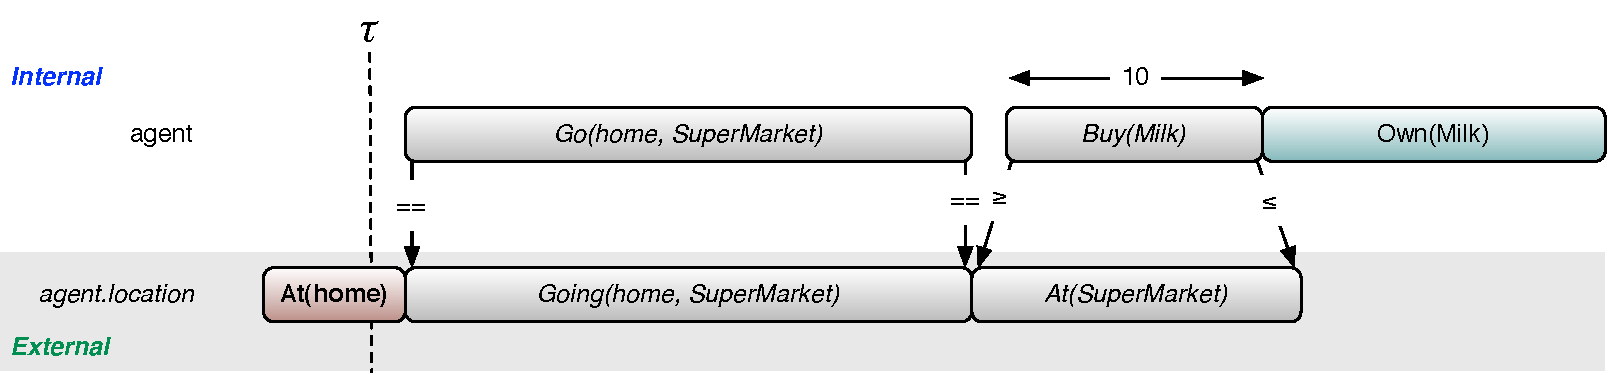
\includegraphics[width=0.7\columnwidth]{figs/shoping_exec_t0}
  \caption{Shopping example : plan produced before synchronization. 
    Tokens in red indicate observations, 
    tokens in blue the goal that this plan attempt to solve. Arrows
    indicate temporal constraints.}
  \label{fig:shop:exec0}
\end{figure}

Now, consider that at the next tick $\tau+1$ the reactor managing the
agent location was able to change the location state varaibale to the
\texttt{Going}. \rx informs our reactor of this new observation which
is added in the plan structure as a fact -- starting exactly at
$\tau+1$ and lastign for an unlknown duration which is at least 1
tick. As this new observation is integrated in the plan through
synchronization the solver can identify the similarity between this
new observation oand the next token in the existing plan. Which mean
that instead of making a blind exhaustive search of all the possible
implication the synchronization process starts its execution with the
assumption that these new observations are consitent with the current
plan maintained. As a result at the end of synchronization we will
have the plan depicted in Fig. \ref{fig:shop:exec1}. Which just
propagated the information provided by the new observation in the
exisiting plan (restricting in turn the start time of \texttt{Going}
and by propagtion of the constraints \texttt{Go} to be {\em exactly}
$\tau+1$). While focusing uniquely on the execution frontier ($\tau+1$
in Fig. \ref{fig:shop:exec1}), the europa solver took benefit of the
exisiting plan to evaluate a solution that asumes that the observation
is consistent with what was decided inside this reactor.


This choice is directed not only by some natural heurisitc choices
made in the solver but even more enforced in general by the heuristic
order of the decision point reolution choices for our {\em internla}
state flaw presented in section \ref{sec:arch:sync} {\em\color{red}
  TODO: need to rework the presentation of thee choices so I can refer
  to them more directly -- algorithm or pseudo theorem should do the
  trick}. Should such a flaw be revealed during synchronization --
meaning that the current state of an {\em internal} state varaibale is
not fully grounded -- the sequencing of the choices will atempt first
a conservative choice in term of maintaining previous state, then an
optimisitic choice in term of the execution/advance in our current
plan to finally attempt other choices that were not predicted by the
model. The two first possible choices are strongly directed by the
exisiting plan which help direct the search within this frame. This
often allow to have a synchronization that is much more directed and
i, in nominal situation such as the one we showed resolve the
deliberation in few steps (often without any backtrack in the search).

\begin{figure}[!htb]
  \centering
  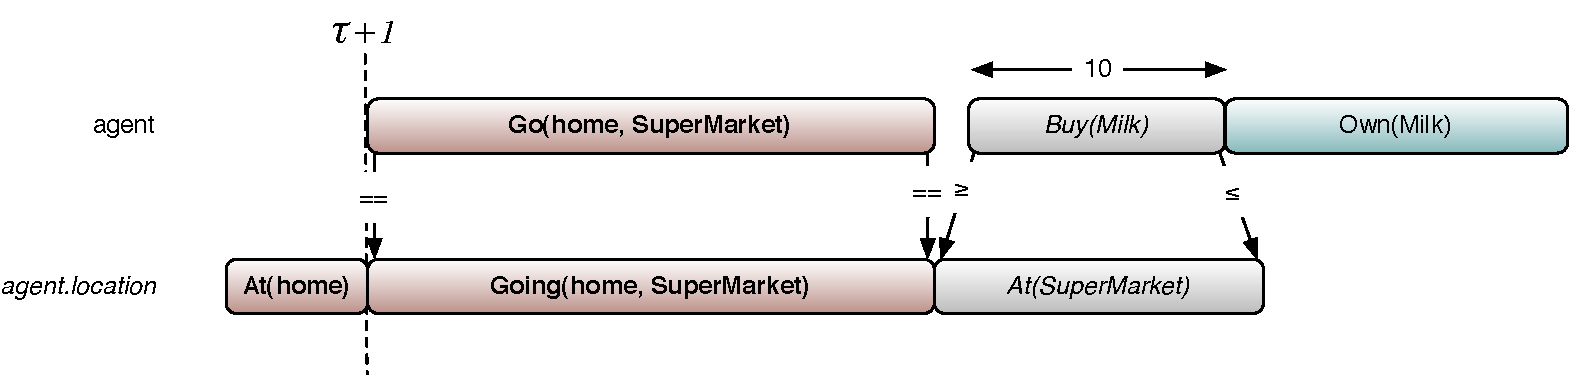
\includegraphics[width=0.7\columnwidth]{figs/shoping_exec_t1}
  \caption{Shopping example : Result of synchronization after the {\em
      Going} observation was received by the reactor with thew plan
    showed in Fig. \ref{fig:shop:exec0}.}
  \label{fig:shop:exec1}
\end{figure}

The synchronization process is also in this process supporting fully
the tracking of the plan execution as it specifies tokens parameters
such as the time points and allow this to propagate through the plan
in order to idenitfy if the plan remains valid -- as in our example --
or that it cannot be executed as it is. The later is often identified
by the synchronization failing to find a consistent solution. for
example dshould the \texttt{Going} observation we receive be to the
\texttt{hardwareStore}, this would break the current plan of our
reactor as we cannot go simultaneously at 2 different places as
illustrated in Fig. \ref{fig:shop:relax}-1. as synchronization is not
possible in this context our strategy is to fully relax all decisions
made by the previous plan steps by just keeping n the plan all the
past observations in both {\em external} and {\em internal} state
variables and the exsiting {\em internal} goals received by this
reactor (\texttt{Own(Milk)} in our example) resulting on the plrtial
plan sghowned in Fig. \ref{fig:shop:relax}-2. In this process the
reactor inform the agent that all {\em external} goals it requested
for the future are note valid anymore which often result in the ownere
of htese timelines to not have to maintain this goal anynmore.

\begin{figure}[!htbp]
  \centering
  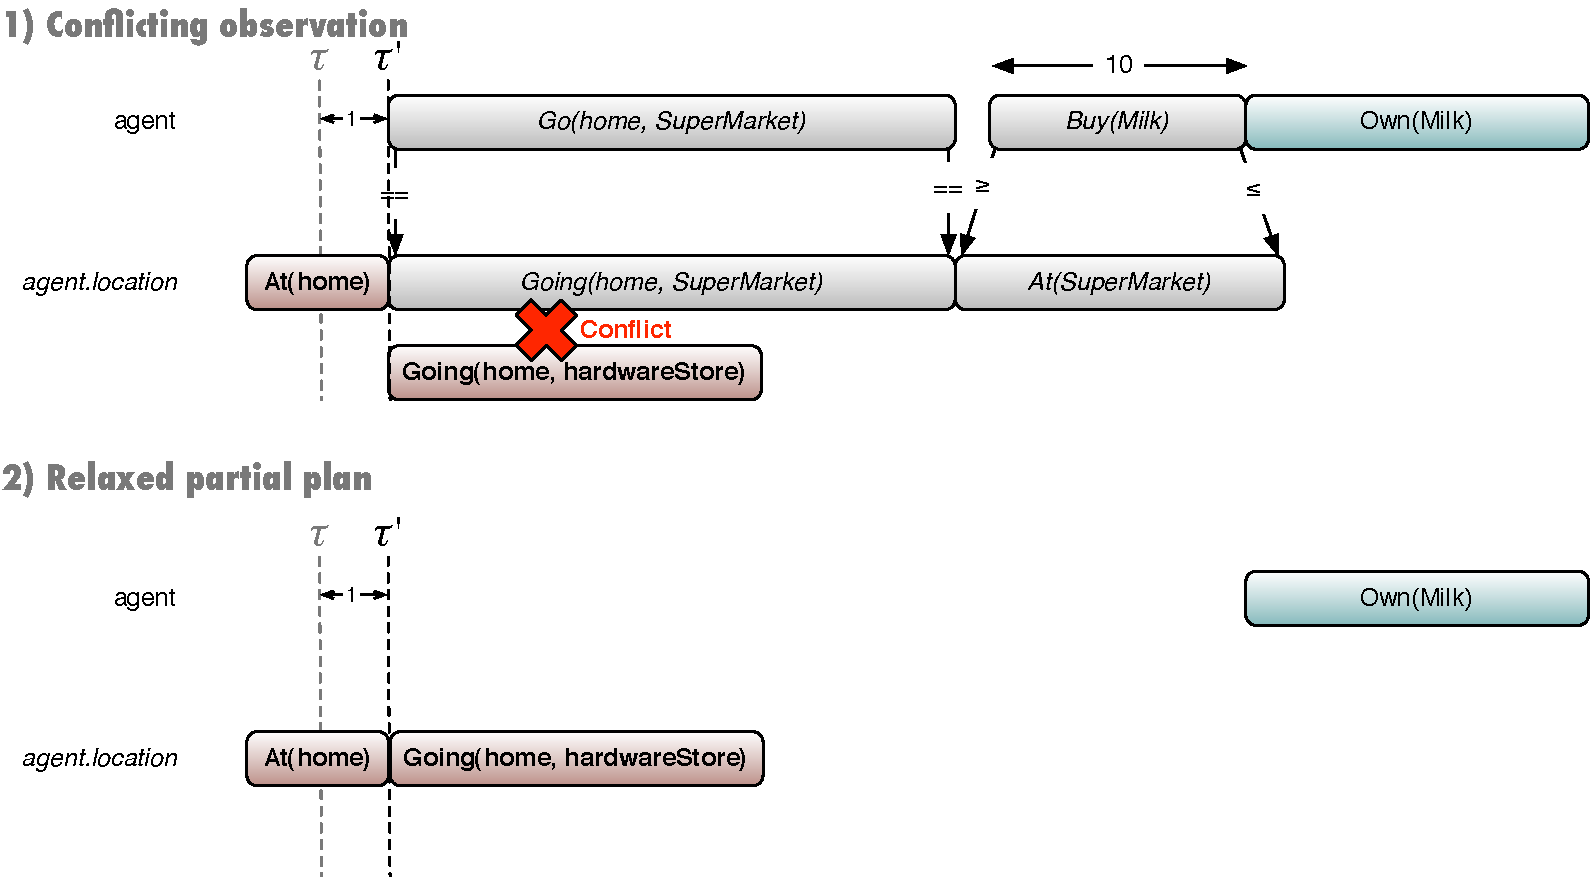
\includegraphics[width=0.7\columnwidth]{figs/shoping_exec_relax}  
  \caption{Illustration of a conflict suring synchronization and the
    resulting relaxed plan for recovery} 
  \label{fig:shop:relax}
\end{figure}

As the plan is not anymore in the way the synchronization can resume
and find a solution as we initial lly described. The newly pending
goals will enforce at the next \texttt{step} to resumed deliberation
on this new fully relaxed partial plan. By the simple use of
synchronization the reactor was not only able to identify that its
plan was not executable anymore but recover from it while offering a
new incomplete partial plan to be resolved during the next
deliberation \texttt{steps}. This on its own ogfer the core
functionality one should except to close the loop between planning and
execution in the sense that synchronization plays the role of what is
typically named as the {\em Executive} in other architectures
{\em\color{red} references to diverse archis, 3-tiered, laas, claraty,
  B Wiliams, and many more}.

In our case though the interaction between planning and execution does
not stop at this level. A core point of the overal schedulling of both
{\em synchronization} and {\em planning} steps resides on our
architecture enforsincing that the synchroniuzation process can occur
in between any step of the plan. This lead us to the fact that not
only synchronization is imnfluenced by the outcome of planning but
this influence goes also in the alternate direction. Specifically when
synchronuiation occuers before we found a complete plan, it will
inject as we described new facts (the {\em external} observations and
resulting {\em internal} state) in the plan database. This
informatiuon will be present when the next planning \texttt{step} will
resume. Therefore they are not intergal part of the plan resolution
(generating potentially new flaws for the planner or contributing to
resolve previously exisiting flaws). The planning process is therefore
perturbed internallyand fully informed on how the world evolves as it
is planning.  This aspect trueluy contrast to other approaches we have
identified in the literature which avoid to perturb the planner during
it search as it is not compatible with the ``off-line planning''
assumption.

By our design choices -- both at the architecture level and the
integration of the europa framework for embedded deliberation -- we
were able to implement an architecture that avoid this limitation
while remaining in a formal frame that still allow for deliberation
and model-based agent control. We believe that this tighter
integration of planning and execution allow the system to ba more
acute of its environment allowing better informaed decision and
tighter reaction. This is possible while still integrating information
such as a long latency for the reactors as long as one can ensure that
synchronization of al the reactors and deliberation steps can be done
in a time that is resonably small in comparison of the agent tick
duration.





% Gives a high-level overview of T-REX, the general design principles and how
% these principles aid in software engineering. Show T-REX block diagram.



%%% Local Variables: 
%%% mode: latex
%%% TeX-master: "setobook"
%%% End: 
